\documentclass[10pt]{article}
\usepackage[utf8]{inputenc}
\usepackage[T1]{fontenc}
\usepackage[english]{babel}
\usepackage{amsfonts}
\usepackage{amsmath}
\usepackage[pdftex]{color,graphicx}
\usepackage{pdfpages}
\usepackage{fancyhdr}
\usepackage{textcomp}
\usepackage{lmodern}
\usepackage{xcolor}
\usepackage{multicol}
\usepackage{soul}
\usepackage{url}
\usepackage{algorithmic}
\usepackage{wrapfig}
\usepackage{caption}
\usepackage{subcaption}
\usepackage{float}
\usepackage{mdwlist}
\usepackage{pgfgantt}
\usepackage[showframe=false]{geometry}
\usepackage{changepage}
\usepackage[bookmarks]{hyperref}
\usepackage{listings}
\usepackage{dirtree}
\pagestyle{fancy}
\usepackage[font=small,labelfont=bf]{caption}
\newcommand{\HRule}{\rule{\linewidth}{0.5mm}}

\def\nosplit{\hfil\penalty 100 \hfilneg \hbox}
\newcommand{\myurl}[1]{\url{#1}}
%\newcommand{\myurl}[1]{\nosplit{\url{#1}}}
\newcommand{\graphicc}[4]{\begin{figure}[H] \centering
            \includegraphics[width={#1\textwidth}, keepaspectratio=true]{{#2}}
            \caption{{#3}} \label{#4} \end{figure}}

% Setup for lstlisting
\lstset{language=C++,
                basicstyle=\ttfamily,
                keywordstyle=\color{blue}\ttfamily,
                stringstyle=\color{red}\ttfamily,
                commentstyle=\color{green}\ttfamily,
                morecomment=[l][\color{magenta}]{\#}
}

%If in need of a header for the document, uncomment this and add desired text!
%\fancyhead[LO,LE]{}
%\fancyhead[RO,RE]{}
%%%%%%%%%%%% END OF PREAMBLE %%%%%%%%%%%%%%%%%%%%%%%%%%%%%%%%%%%%
\begin{document}
\begin{titlepage}

\begin{center}

\textsc{\LARGE Project Report}\\[1.5cm]

\textsc{\Large DIKU Bachelor project}\\[0.5cm]

\HRule \\[0.4cm]

{ \bfseries Visualizing Chan-Vese segmentation results through the DSC datastructure in Autodesk Maya }\\[1cm]

\HRule \\ [7.5cm]

% Author and supervisor
\begin{minipage}{0.5\textwidth}
\begin{flushleft} \large
Author:\\
Martin Jørgensen (tzk173)\\
\textit{martinnjorgensen@gmail.com}\\
\vspace{0.5cm}
\end{flushleft}
\end{minipage}
\begin{minipage}{0.4\textwidth}
\begin{flushright} {\large
\textbf{\today} }\\
Supervisor(s):\\
Kenny Erleben (kenny@diku.dk)\\
Ulrik Bonde (bonde@diku.dk)
\end{flushright}
\end{minipage}

\vfill

% Bottom of the page front page


\end{center}

\end{titlepage}
\clearpage

% Abstract
%TODO: Make this look pretty and write it... duuh.. :P
\hspace{1cm}\\[5cm]
{\huge Abstract}
\\\HRule\\

The Image-group on DIKU currently work with a number of simulations and mesh
structures, each requiring a custom tool for visualization. It is the wish that
a new tool be created to unify the visualization process.

The design developed in this project, visMesh, is a C++ plugin for Autodesk Maya
that includes a simple virtual interface for plugging in both new simulators and
mesh structures. A prototype of the plugin was developed and tested using a
discretized 3D Chan-Vese segmentation library and the DSC mesh framework.

The prototype was tested and compared to the current OpenGL application that is
used to visualize the Chan-Vese segmentations. The comparison was based on
visualization results, CPU- and memory usage both during simulation and when
only displaying the results.

The prototype was found to solve a number of the problems with the current
OpenGL solution, amongst others: rendering simulations as films, low framerate
with complex meshes and stepping back and forth in a simulation. Since the
prototype is not feature complete, a number of improvements have been suggested
to increase the usability of the tool.\\
\HRule
\newpage
\tableofcontents
\newpage

% Introduction
\section{Introduction}

For my bachelors project I helped DIKUs Image-group by designing and
prototyping a tool to help them visualize simulations and mesh
structures. Currently their only way of visualizing their research are in a crude
OpenGL applications that are written specifically for each project.

My supervisors are currently working with image segmentation in the form of a
Chan-Vese model based segmentation algorithm and a moving mesh framework called
Deformable Simplicial Complexes (from here on just called DSC), so my project
will be centered around creating a visualization tool for those two projects
that can be adapted to fit any other project.

The implementation of the project will be in the shape of a Autodesk Maya plugin,
which will allow the user to visualize the results of their simulation and
easily provide parameters for the simulation to observe changes. These
visualizations can be used both internally to help debug an algorithm or be
rendered to images or animations that can be published.

\graphicc{0.5}{img/not_so_pretty_mix.png}{A mix of two pictures rendered in the
resulting Maya plugin. The shape is loaded from a DSC file into the simulator,
a shader have then been applied to the shape. The left image is
rendered with Mayas default software renderer, the right one is rendered with Mayas
Mental Ray renderer.}{fig:intro}

In this report I will first go over the theoretical knowledge needed to complete
the plugin The DSC framework and what Simplicial Complexes are, and then
move on to explain the Chan-Vese segmentation algorithm and how Autodesk Maya
works. Afterwards I will cover my analysis of the problem and the design of a
solution. The report will then describe the actual implementation of the plugin
and the use of CMake to make future work and usage easier.

Finally I will go over the results of the plugin and compare them to the
current OpenGL solution and go over the changes that should be done in order to
further improve the solution.

The code can be obtained by writing to either me, Kenny or Ulrik (see frontpage
for emails.)

%Fra Torbens slide:
%En indledning er:
%En kort teaser, som for den forventede læser gør rede for, hvorfor projektet er in-
%teressant, for state-of-the-art, for jeres resultater, og for forventninger til læseren.
%
%Tænk: Hvis en teknisk projektleder eller en studiekammerat skal læse indledningen
%(men ikke resten af rapporten), hvad skal vedkommende da læse for - overordnet
%- at forstå jeres projekt?

% Descripe the problem we want to solve
\section{Problem Description}
This section will outline the general problem that that I have attempted to
solve during the course of this project.

The goal of the project was to design and implement a piece of software that researchers in
the Image-group could use to visualize the results of a Chan-Vese segmentation.
This visualization was implemented as a plug-in for Autodesk Maya, a
professional 3D program.

The actual image segmentation is performed by a piece of software that Ulrik
Bonde wrote, which I have been granted access to. The output data from this
software is a moving tetrahedral mesh maintained by the DSC framework.
Chan-Vese and DSC is described in sections \ref{sec:chanvese} and \ref{sec:dsc}
respectively.

The current method for visualizing the results of the segmentation is a
simple OpenGL application that offers very little in the way of customization
or render options. By switching to Maya, the researchers will gain an extremely
powerful new render engine.

In order to provide the researchers with a new tool they can use, I should
implement a plugin for Maya that gives a simple GUI for retrieving the
segmentation data and tweak the segmentation itself without having to actually
leave Maya at any point.

The rest of this report assumes the reader to be at least on-par with a
bachelor in computer science or similar education.

% Background knowledge
\section{Deformable Simplicial Complexes}
\label{sec:dsc}

This section will describe the DSC framework and the theory it's built upon.

\subsection{Simplices}

A simplex (simplices in plural) is a generalisation of the notion of a triangle
to an arbitrary number of dimensions. The triangle is as such a 2-simplex and it
is the convex hull of its three vertices. More formally we can state a
$n-$dimensional simplex (a $n-$simplex) as the convex hull of its $n+1$
vertices, furthermore a $n$-simplex contains $n+1$ ($n-1$)-simplices, the
exception being the 0-simplex which is the lowest dimensional simplex.

\begin{figure}[h!]
        %====================
        % TODO: Fix this figures, its not pretty :(
        %====================
        \centering
        \begin{subfigure}[b]{0.1\textwidth}
                \includegraphics[width=\textwidth]{img/0simplex.png}
                \caption{A 0-simplex. (point)}
                \label{fig:0simplex}
        \end{subfigure}%
        \qquad
        \begin{subfigure}[b]{0.2\textwidth}
                \includegraphics[width=\textwidth]{img/1simplex.png}
                \caption{A 1-simplex. (line)}
                \label{fig:1simplex}
        \end{subfigure}
        ~
        \begin{subfigure}[b]{0.3\textwidth}
                \includegraphics[width=\textwidth]{img/2simplex.png}
                \caption{A 2-simplex. (triangle)}
                \label{fig:2simplex}
        \end{subfigure}%
        ~
        \begin{subfigure}[b]{0.2\textwidth}
                \includegraphics[width=\textwidth]{img/3simplex.png}
                \caption{A 3-simplex. (tetrahedron)}
                \label{fig:3simplex}
        \end{subfigure}

        \caption{The four different simplices that are drawable in three dimensions.
                 The 0- and 1-simplex is technically not drawable, but are shown
                 here for clarification.}
        \label{fig:simplices}
\end{figure}

Figure \ref{fig:simplices} illustrate the four simplest simplices:
\begin{itemize}
  \item \textit{0-simplex:} This is a point in a 0-dimensional universe. When
    pulled into a multidimensional universe, it will usually be represented as a
    vertex.

  \item \textit{1-simplex:} This simplex is seen as a straight line with no
    other properties than length. It contains two 0-simplices.

  \item \textit{2-simplex:} The 2-simplex is a triangle, it exists as a
    2-dimensional figure with no "thickness" it is the lowest dimensional
    simplex to have a surface. It contains three 1-simplices.

  \item \textit{3-simplex:} This simplex is called a tetrahedron, it is the
    lowest dimensional simplex to have a volume and not just a surface. It
    contains four 2-simplices.
\end{itemize}



% During this project the most Important simplex is the 3-simplex because I will
% be working with a 3-dimensional mesh, but it is relevant to explain that
% simplex can have an arbitrary number of dimensions and that all simplices
% actually consist of simplices of a lower dimension.

Further definitions on simplices and sets of simplices can be made.
The dimension of a set of simplices $\Sigma$ is the maximum dimension of any
simplex in it. This is formalized as
\[
    \text{dim}(\Sigma) = \text{max}\{\text{dim}(\sigma) | \sigma \in \Sigma \}.
\]
We also define the $k$-subset as a set of all $k$-simplices in $\Sigma$ as
\[
    \text{filter}_k = \{\sigma_i \in \Sigma | \text{dim}(\sigma_i) = k\}.
\]

\subsection{Simplicial Complexes}
Simplicial complexes are groups of simplices that are grouped together to yield
a more complex structure. In order for a group of simplices $\Sigma$ to form a
simplicial complex it will need to satisfy two conditions:
\begin{enumerate*}
    \item $\Sigma$ is closed, such that for any simplex $\sigma \in
          \Sigma$ all the faces of $\sigma$ are in $\Sigma$.

    \item The intersection of any two simplices $\sigma_i \cap
          \sigma_j$ for $\sigma_i,\sigma_j \in \Sigma$ must be a face of both
          $\sigma_i$ and $\sigma_j$.
\end{enumerate*}

Figure \ref{fig:scexamples} shows a simplicial complex and a group of
simplices that do not constitute a simplicial complex since they do not satisfy
the above conditions.

\begin{figure}
        \centering
        \begin{subfigure}[b]{0.4\textwidth}
                \includegraphics[width=\textwidth]{img/wiki_simplcialcomplex.png}
        \end{subfigure}%
        \qquad
        \begin{subfigure}[b]{0.3\textwidth}
                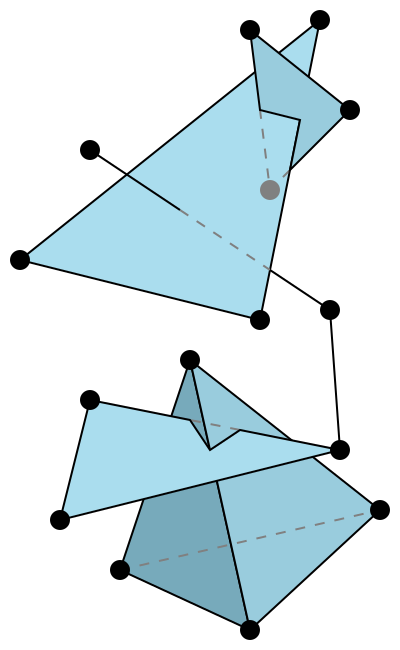
\includegraphics[width=\textwidth]{img/wiki_nonsimplicialcomplex.png}
        \end{subfigure}

        \caption{A valid simplicial complex(left), and a set of simplices
                 that do not qualify as a simplicial complex (right.) Source:
                 Wikipedia.org \cite{wikisc}}
        \label{fig:scexamples}
\end{figure}

%Reinsert this if it is needed for later understanding.
%For any Simplicial complex $K'$ that is a subset of another simplicial complex
%$K' \subset K$ is called a subcomplex of $K$.

In order to later work with a simplicial complex, it is beneficial to
define a number of topological relations for the simplices in a complex. For a
$n-$dimensional simplex $\sigma^n$ in a simplicial complex $K$ we define:
\begin{itemize}
    \item \textit{Boundary}: For $p > q$ the boundary relation is the set of
         $q$-faces of $\sigma^p$ defined as
         \[
            B_ {p,q}(\sigma^p) = \text{filter}_q\{\sigma \in K | \text{vert}(\sigma) \subset \text{vert}(\sigma^p)\}.
         \]

    \item \textit{Coboundary}: For $p < q$ the Coboundary relation is the set of
         all $q$-simplices that have $\sigma^p$ as a face, defined as
         \[
            C_ {p,q}(\sigma^p) = \text{filter}_q \{\sigma \in K | \text{vert}(\sigma^p) \in \text{vert}(\sigma)\}.
         \]
    % Reinsert if needed later
    %\item[Adjecency] for $p >0$ the adjecency relation is a set of all
    %     $p$-simplices which share a $p-1$-face with $\sigma^p$:
    %     \[
    %        A_p(\sigma^p) = filter_p\{\sigma \in K : |vert(\sigma^p) \cap vert(\sigma)|=p\}
    %     \]
\end{itemize}

We will now use these to define the \emph{star}, \emph{link} and \emph{closure}
of a simplex $\sigma$.

The star of a simplex $\sigma$ is the set of all simplices in $K$ which have
$\sigma$ as a face (for illustration see Figure \ref{fig:star})
\[
  \text{star}(\sigma^p) = \{ \sigma \in K | \text{vert}(\sigma^p) \in \text{vert}(\sigma) \} = \bigcup_{q=p+1}^{n}C_{p,q}(\sigma^p).
\]
\graphicc{0.6}{img/wiki_star.png}{The star(green) of one simplex(yellow).
Source: Wikipedia.org \cite{wikisc}}{fig:star}

We also define the closure of a simplex $\sigma^p \in K$ as the set (for
illustration see Figure \ref{fig:closure})
\[
  \text{closure}(\sigma^p) = \bigcup_{q=0}^{p}B_ {p,q}(\sigma^p).
\]
\graphicc{0.6}{img/wiki_closure.png}{The closure(green) of two simplices
(yellow). Source: Wikipedia.org \cite{wikisc}}{fig:closure}

Finally we define the link of a simplex (for illustration see Figure \ref{fig:link}) as
\[
  \text{link}(\sigma) = \text{closure}(\text{star}(\sigma)-\text{star}(\text{closure}(\sigma))).
\]
\graphicc{0.6}{img/wiki_link.png}{The link(green) of one simplix(yellow).
Source: Wikipedia.org \cite{wikisc}}{fig:link}

Both the star- and closure-operation can be defined as the union of the results
of running the operation on each subsimplex formally expressed as
\[
  \text{star}(\Sigma) = \bigcup_{\sigma_i \in \Sigma} \text{star}(\sigma_i)
\]
and
\[
  \text{closure}(\Sigma) = \bigcup_{\sigma_i \in \Sigma} \text{closure}(\sigma_i).
\]


\subsection{Deformable Simplicial Complexes}
DSC is a framework for 3D tetrahedral meshes which supplies a set of operations
and promises to always optimize its mesh. DSC works inside a ``computational
domain'', this domain further contains a number of sub-domains that are either
\textit{inside} (a mesh in the world) or \textit{outside} (the volume around the
mesh.) DSCs domain is a tetrahedral mesh (a simplicial complex) that satisfies
the two criteria
\begin{itemize}
  \item \textit{Simplicial Complex Criterion:} The intersection between two
        simplices must be either empty or their common face. For a tetrahedron,
        that is the common face, edge or vertex.
  \item \textit{Conform To Interface:} The interface of a DSC is a set of
        boundary vertices/edges/faces between simplices that are marked as being
        either inside or outside.
\end{itemize}

This allows the DSC framework to contain several meshes in its domain (several
\textit{inside} sub-domains.) and let them merge together into a single domain.
Figure \ref{fig:meshmelt} shows an example of two domains melting together to
form a single domain. The example is drawn in 2 dimensions for clarity.

\graphicc{1.0}{img/mesh_melt.png}{Two domains melting together to form a single
domain. Blue simplices are inside, grey are outside.
Source: Misztal\cite{DSC10}.}{fig:meshmelt}

Part of the merging process is moving the vertices. On p. 50 of \cite{DSC10}
\texttt{Algorithm 4} and \texttt{Algorithm 5} describes how DSC moves vertices
around. When moving a vertex, DSC will calculate if the move will cause the
vertex to intersect with any simplex that is in the \textit{link} of the vertex.
If there is an intersection the vertex will be moved to the intersection, if
there is no intersection, the vertex will be moved the full length. This is
seen on Figure \ref{fig:meshmelt} where a vertex moves into contact with an
edge that is part of its \textit{link}.

One of the benefits of the DSC framework is that it will automatically make
sure that all of its tetrahedrons have a certain quality. DSC ascertain its own
quality by looking at the quality of the worst tetrahedron in the mesh as well
as seven threshold means (p. 34 \cite{DSC10}). A quality mean
$\overline{q}_\theta$ with the threshold $\theta$ is computed as
\[
  \overline{q}_\theta = \frac{1}{\text{No. of tetrahedra in M}}
  \sum_{t \in M}^{}(\text{min}(q(t),\theta)),
\]

where $M$ is the mesh and $q$ is the tetrahedron quality measure. The seven
different thresholds used in DSC are: $sin(1^\circ)$, $sin(5^\circ)$,
$sin(10^\circ)$, $sin(15^\circ)$, $sin(25^\circ)$, $sin(35^\circ)$ and
$sin(45^\circ)$. Using a broader measurement over all the tetrahedra instead of
just going with the quality of the worst tetrahedron yields a better overall
assessment of the mesh, and reflects better if the mesh is being optimized since
the worst tetrahedron may not have been optimized. The mesh optimization loop
of the mesh will terminate if either the worst tetrahedron improves or one of
the thresholds improves by at least $0.0001$.

The mesh improvement algorithm used by DSC is described as \texttt{Algorithm 1}
in pseudocode on p. 55 of \cite{DSC10}. DSC will first run a vertex smoothing
pass and a topological pass on the mesh. After this it will enter a loop that
will not break until it have made three iterations where the mesh have not improved
sufficiently. For each pass it will attempt a vertex smoothing pass, a
topological pass and a thinning pass. The Topological pass is described as
\texttt{Algorithm 2} on the same page, and the thinning pass is described as
\texttt{Algorithm 3} on p. 56 of \cite{DSC10}. The vertex smoothing algorithm
is called \textit{Laplacian Smoothing} \cite{wikils}. It works by adding all
the neighbours of the node we want to smooth, and dividing the resulting vector
by the number of neighbours
\[
  \overline{x_i} = \frac{1}{N}\sum_{j=1}^{N}x_j,
\]
where $\overline{x_i}$ is the new position of the vertex, and $N$ is the number
of vertices addjecent to $x_i$.

The topological pass will try to take each edge and face of all the tetrahedra
and attempt to remove it using its built-in edge removal algorithm and
multi-face re-triangulation.

The thinning pass will go over all the edges in the mesh and attempt to collapse
it. It will first try and collapse its vertex $b$ into the vertex $a$, and
smooth the position of $b$. If this does not work, it will attempt to collapse
$a$ into $b$ and smooth $b$.
\section{Segmentation}
\label{sec:chanvese}
The segmentation will be handled by the Chan-Vese method for image segmentation.
This is a segmentation method that builds on the Level-Set method, which will
also be explained in this section.

\subsection{Level-Set Method}
The level-set method is a method for tracking shapes or, in our case, interfaces.
The level-set method uses a numerical function to determine whether a point is
in the shape, on the interface or outside without doing any parameterization of
the edge. This proves valuable if the shape creates ``holes'' or merge with
other shapes as no reparameterization is needed.

In a 2D universe the level set method would then give us a curve $\Gamma$ that
is the interface or edge in a figure. Doing this will require a helper function
$\psi$ that can decide whether a given point is inside, on the shape or outside.
The level-set method for the interface looks like this
\[
  \Gamma = \{ (x,y)|\psi(x,y)=0  \},
\]
assuming that $\psi$ returns 0 for any point on the interface. Extending $\psi$
to have specific values for points inside or outside can increase the
usefulness of the method. The challenge is to design a $\psi$ that gives useful
data for a desired input.

\subsection{Chan-Vese Segmentation}
The Chan-Vese segmentation method is an image segmentation that uses the
Level-Set method along with an energy function as $\psi$ to find and track
contours in images. For a bi-level image where every pixel have a value of 0 or
1, the Heaviside function can be used as $\psi$, giving all the pixels that are
inside the shape:
\[
  H(x) = \left\{
  \begin{array}{l l}
    1 & \quad x \geq 0 \\
    0 & \quad x = 0
  \end{array}
  \right.
\]

In order to track an interface, further modification is needed. This could be
done by doing a comparison of the surrounding pixels. If the pixel in question
is touching a pixel of value $0$, but is itself valued $1$, it would be on the
interface. The $\psi$ function can then be expanded to return different values
depending on the location of the pixel (See Figure \ref{fig:cv-interface} for
an example.)

\graphicc{0.5}{img/cv-interface.png}{Here the $\psi$ function returns 0 for
pixels on the interface, $>0$ for pixels inside and $<0$ for pixels outside. Source:
Chan and Vese \cite{cv01}}{fig:cv-interface}

Energy functions are proposed in both \cite{cv01} and \cite{rc09}. They have the
same basic structure, that consist of four weighted terms. Each term represent a
feature of the image. The first term is the length of the edge. It is used to
enforce a penalty for longer or short edges, allowing more detailed edges. The
second term enforces a penalty for the area covered by the inside domain
allowing us to change how much area we want inside the shape. The third and
fourth term share a purpose, they work with the uniformity of the
pixel-intensity of the for- and background of the image, respectively.

Since the segmentation model I will work is modified to work on a 3D tetrahedral
mesh. The first term is changed to weigh surface area.
The second term weigh volume, and the third and fourth use a function that
interpolates image values from the vertices of a tetrahedron. The complete
energy function (from \cite{chanveseposter}) for the contour C is
\begin{align*}
  \text{Ê}(C) = &\mu \sum_{\alpha \in C}^{}A_\alpha \\
  &+ v \sum_{\beta \in \Omega_{in}}^{} V_\beta \\
  &+ \alpha_{in} \sum_{\beta \in \Omega_{in}}^{}\left(\text{Û}(p_\beta) - c_{in}  \right)^2 V_\beta \\
  &+ \alpha_{out} \sum_{\gamma \in \Omega_{out}}^{} \left(\text{Û}(p_\gamma) - c_{out} \right)^2 V_\gamma \\
\end{align*}

%==============================================================================
%TODO: Find the original CV article its [1] in cr09 and use that as reference?
% A fitting energy functional for a segmentation of images have been written in
% \cite{rc09}. I will show it here to provide an insight into the complexity of
% the segmentation algorithm but offer no greater discussion on it since it
% is far beyond the scope of this report. Before showing the functional itself a
% few symbols must be established:
% \begin{itemize*}
  % \item We again use the Heaviside function $H$.
  % \item $I$ is the image to be segmented.
  % \item $\Omega$ is the domain of $I$.
  % \item $p,v,\lambda_1$ and $\lambda_2$ is parameters for the function, set
        % depending on what type of image you wish to segment.
  % \item $c_1$ and $c_2$ is the averages in the regions of $I$ where $\phi \geq
        % 0$ and $\phi < 0$. They're given as:
        % \[
          % c_1 = \frac{\int_\Omega I\cdot H(\phi) dx dy}
                     % {\int_\Omega H(\phi) dx dy}
          % ,
          % c_2 = \frac{\int_\Omega I\cdot (1-H(\phi)) dx dy)}
                     % {\int_\Omega (1-H(\phi)) dx dy}
        % \]
% \end{itemize*}

% This taken into account the full functional will be:
% \begin{align*}
  % F(\phi) = &\mu{\Big(}\int_\Omega|\nabla H(\phi)| dx{\Big)}^p\\
            % &+ v\int_\Omega H(\phi) dx\\
            % &+ \lambda_1 \int_\Omega |I-c_1|^2 H(\phi) dx\\
            % &+ \lambda_2 \int_\Omega |I-c_2|^2 (1-H(\phi)) dx
% \end{align*}

% The functional can be though of as four terms with their specific purpose:
% \begin{itemize*}
  % \item The first term will say something about the penalty put on the length of
        % the edge for the segmentation. If a short edge is expected this should
        % be set heavier than if a long intricate edge is expected.
  % \item The second term is a penalty applied to the area of the segmentation, so
        % if the result is expected to have a low area, this should be weighted
        % heavier.
  % \item The third and fourth term share a purpose, they work with the
        % uniformity of the pixel-intensity, of the fore- and background of the
        % image respectively.
% \end{itemize*}
% Description of the Maya DG and DAG. Other theoretical Maya things according to learning goals.
\section{Autodesk Maya}
\label{sec:Maya}
The section will describe the way Autodesk Maya represents data internally and
what we can do to be able to add our own code into the program through the
plugin system.

\subsection{Internal Representation}
Maya represents all objects and operations in two internal graphs with different
characteristics and purposes, the Dependency Graph (DG) and
the Directed Acyclic Graph (DAG).

\subsubsection{Dependency Graph}

%TODO: meshes can be data in plugs, shapes are what is displayed.
The DG is a directed graph consisting of a number of nodes. Nodes in the DG can
have a number of attributes (called plugs) that can be used as either
\textit{input}, \textit{output} or \textit{unconnectable}. The
\textit{input/output} nodes define relationships between objects in Maya. All
objects and modifiers in Maya is represented in the DG as one or several nodes.

An example could be a map-displacement modifier with three input plugs and one
output plug. Input plugs would be mesh data (not a mesh object, but simply the
data needed to create one), an input displacement-map and an integer deciding
strength. The output plug will then deliver mesh data that can be used as input
to another modifier, or to render an actual mesh. Connectivity to such a node
would then be that all other nodes that needs the output mesh data connects to
the output plug and request the mesh data there. The input mesh data plug will
need to be connected to a DG node that can provide a base mesh the modifier can
work on. The integer plug can be set to be visible in the UI, so a user can
specify it through a text/numeric-input field.

In order to maintain consistency through the graph, plugs can be marked
\textit{dirty}. If, for instance, we change the strength plug of the displacement
node discussed before, the output plug will be marked dirty, and Maya will in
turn mark all plugs that read the output plug as dirty, propagating the change
across the entire DG. If any dirty plug is requested it will be recalculated. If
any of its input plugs are dirty, they will propagate the recalculation request
through the graph again. This way Maya only ever updates nodes if it has to.

There can be several reasons for plugs to become dirty, and for them to be
requested again. Plugs become dirty when they are unplugged/plugged-in (the DG
can change as nodes are added), keyframes are changed or other attributes are
modified. The most common reason a plug is called to be recalculated, is when a
renderer calls for the final result of the DG.

\subsubsection{Directed Acyclic Graph}

Whereas the DG nodes usually is objects and modifiers in the Maya scenes, the
DAG nodes are transformation nodes, locator nodes and similar unrenderable
operations. DAG nodes specify operations to be performed inside the 3D space
such as translation and rotation. DAG nodes are usually set as parents of DG
nodes but these connections are not normally apparent.

\graphicc{1}{img/dagdg-example.png}{An example scene in Maya with a single
  object, a number of modifiers and dataflow- and relationship arrows.}{fig:dagdg}

Figure \ref{fig:dagdg} shows an example scene in Maya, where a DG node that
generates geometry based on user input provides a mesh for a surface noise
generator. The generator outputs a mesh that the viewport, production renderers,
or any other DG node that wishes so, can pull. Scale- and rotation transformation
modifiers have been provided. The solid arrows represent data flowing through
the graph, the dashed ones represents relationships; a parent will point to its
child.

\subsection{Plugin System}
\label{sec:pluginsystem}
Maya allows for several different forms of customization:
\begin{itemize}
  \item MEL-scripts (Maya Extended Langauge)
  \item Python-scripts (interpreted within Maya itself.)
  \item External python plugins through Mayas own modules.
  \item C++ Maya plugins compiled and linked as dynamic libraries.
\end{itemize}

I will be writing a plugin using C++. This language was chosen for three reasons:
both the DSC and Chan-Vese codebase I will be integrating with is written in
C++, and the people that will use the plugin already have experience with C++
which makes it easier to take over once my project have ended. Finally C++
can be an extremely efficient language if written properly, providing only a
minimum of overhead for the link between simulator and plugin.

A C++ plugin gets compiled to a dynamic library, which on windows is called
\textit{.mll} (this is actually a DLL file) and have two exported entry points
called \texttt{initializePlugin} and \texttt{uninitializePlugin} which Maya will
call when registering and deregistering the plugin respectively.

% Fluff for implementation
%\input{analysis.tex} % 08-10-2013: Deprecated for a unified approach
%\input{design.tex} % 08-10-2013: Deprecated for a unified approach
\section{Analysis and Design}
This section of the report covers the analysis of the problem and the design of
a solution to this problem. It includes decisions about premake systems, 3D
applications and the design of a mesh- and simulator interface.

\subsection{Platforms}
\label{sec:platforms}
% Platform stuff (Why: Cmake, Maya, C++)

A general wish for the visualization system is that it should be platform
independent. To avoid having to maintain 2-3 different build profiles such as
a Unix Makefile, Visual Studio project and XCode project, or similar files, a
premake system had to be chosen.

As choices for the premake system three pieces of software came up:
\begin{enumerate*}
  \item Premake - \myurl{http://industriousone.com/premake}
  \item CMake - \myurl{http://www.cmake.org/}
  \item SCons - \myurl{http://www.scons.org/}
\end{enumerate*}

All three systems are free and promise total compatibility with all the operating
systems. Both Premake and CMake uses their own syntax to define projects while
SCons uses python, which gives great flexibility when it comes to configuring
the project since it allows full use of the python language. The existing
libraries (Chan-Vese and DSC) both used CMake as premake system, giving a strong
incentive to continue using it.

Since I would need to link/include a lot of files from Mayas devkit in order to
complete the plugin, an automatic way of detecting the Maya location was needed.
Neither SCons or Premake had any built-in or user supplied features that allowed
this, but a CMake user created and shared one such module\footnote{\myurl{
https://github.com/frarees/Maya-cmake}}. As long as the Maya install directory
is standard, it will work just fine.

Since I had no prior experience with any of the systems, and they seem like they
have a similar learning curve, the decision of a premake system was based on
the ability to find Maya by itself, and the preferences of the researchers that
will maintain the plugin afterwards. In the end CMake was chosen as a premake
system in order to smooth out interacting with existing projects.

There is a number of 3D modelling programs available, but I only have experience
with a small number of them. Additionally the researchers had previous
experience with Autodesk Maya. This, and the fact that Maya ships for both
Windows, Linux and OS X lead to the selection of Maya as the framework for the
visualization plugin.

% There is only very few widely used 3D modelling programs in general, and even
% fewer that are actually available on several platforms. There was not strong
% opinion on choice of software from the researchers, but they did have experience
% with Maya from previous projects, so it was selected as the framework for the
% visualization plugin.

% As written in Section \ref{sec:pluginsystem} there is a choice of languages
% involved in creating a Maya plugin. For this project C++ was chosen because it
% is a very efficient language when written properly, and both the DSC and
% Chan-Vese libraries are written in C++, which will make integrating them a lot
% easier.

\subsection{Simulation}
\label{sec:sim}
The original goal of the plugin was to create a new way to visualize and animate
the steps and result of a Chan-Vese image segmentation without having to do it
in a custom-made OpenGL application, as is the current solution. The primary
input for the plugin will be meshes extracted by the provided Chan-Vese library.

It was, however, decided early in the project that if it was possible to make a
more uniform interface towards the plugin so that the Chan-Vese segmentation
might be replaced by any other simulator. This would be a preferable solution.

With that in mind we have to find a way that allows for an arbitrary simulator
to be used in the plugin. The original plan was to ``hardcode''
the interaction of the simulation into the plugin itself. This will not satisfy
a generic method of simulation, since that would require a significant code rewrite
every time the simulator was replaced. This leaves two ideas for integration:
\begin{enumerate*}
  \item Dynamically loading the simulator into the plugin, similar to the way Maya
    loads plugins.
  \item Create a ``interface'' specification/API that allows for an easier
    integration, though not fully automatic.
\end{enumerate*}

The first solution is by far the most optimal for the user, but designing and
implementing a way to dynamically load and unload code is a complex task, especially
considering my time constraints and the fact that the plugin should work on both
Linux, OS X and Windows.

%The second solution is based in the same principle of virtual interfaces as the
%virtual file system interface in the BUENOS kernel. Basically the a small class
%should be supplied that overrides a given class specification that is shipped
%with the plugin. An example here would be a header containing:

The second solution is less optimal for the user but is significantly less
complicated to implement. The idea is to implement an interface with a uniform
way for a user to provide a new simulator. This is basically a C++ header file
that specifies a set of methods that the simulator must provide in order to work
with the plugin. This is the method I chose for the design in order to keep the
project at a level I could realistically finish in time.  An example of such a
header file can be seen here:
\begin{lstlisting}
[...]
class simulator {
public:
  virtual void  initialize() = 0;
  virtual mesh* getMesh() = 0;
  virtual void  step() = 0;
}
[...]
\end{lstlisting}
To add a new simulator into the plugin the class will then just need to be
implemented, similar to this:
\begin{lstlisting}
#include <simclass.h>

class mySim : public simulator {
  void  initialize() { [...] };
  mesh* getMesh() { [...] };
  void  step() { [...] };
}
\end{lstlisting}
The new \texttt{mySim} class will do the actual conversion from whatever
input/output the simulator needs and into the specs of the plugin. The above is
a simplified example; a way to pass multiple arguments to the simulator should
be specified.

This approach would mean that the plugin must be recompiled in order to fit a
new simulator, and it would be unable to fit several simulators at once. These
are however acceptable trade-offs, since the wish to add a generic simulator
approach was not part of the original plan.

The interface should provide a set of functions that allow for some control.
The current implementation will need the following set of functions:
\begin{itemize}
  \item \texttt{Initialize}: A call that allows the plugin to initialize the
    simulator. After this call, the simulator should be ready to work. This
    function should include a method that allows for the plugin to pass
    parameters to the simulator.
  \item \texttt{getMesh}: This method should return a mesh to the plugin in some
    mesh format The mesh should correspond to the current state of the
    simulation.
  \item \texttt{step}: A method that causes the simulator to simulate a new
    timestep. This method should be overrideable with a version that takes
    ``step-size'' as an argument, giving finer control of the simulation.
  \item \texttt{getArguments} This method returns an array of strings that are
    the names of the simulation parameters. This is meant to allow the user to
    tell the plugin what sort of parameters it needs. The input from these
    parameters will be used to initialize the simulator.
\end{itemize}

\subsubsection{Chan-Vese}
Since the specific goal of this project was visualizing results from a Chan-Vese
image segmentation, an interface for the Chan-Vese simulator will need to be
created.

The Chan-Vese library itself provides very simple and clean access. Currently it
can be ``warm-started'' from any DSC mesh by loading it into the library at
runtime. It also allows for direct extraction of a segmentation using a single
function call. These simple ways to interact with the simulator will make
the virtual simulator class even simpler to write.

How to use the DSC data extracted from the simulator is covered in Section
\ref{sec:data}.

\subsection{Datastructure}
\label{sec:data}
As with the simulator it was a wish that the plugin could have its internal mesh
structure changed without significant work. This leads to me designing an
additional interface, using the same integration strategy as with the simulator.

Again, this is not a strictly needed feature, but would improve the usefulness
of the plugin greatly as it will allow researchers to change mesh structures as
often as they wish. This is especially useful when the simulator is changed,
since it might not be using a DSC mesh but some entirely new mesh structure.

Just like with the simulator we wish to create a class definition that allow
future users to create easy bridges into the plugin. Such an interface should
have the following functionality:
\begin{itemize}
  \item \texttt{vertices}: The mesh should provide a way to access its vertices.
  \item \texttt{faceCounts}: Access to an array of integers telling how many
    points are part of each face.
  \item \texttt{faceConnects}: Access to an array of integers telling which
    verts are part of each face.
  \item \texttt{save/load}: The mesh should preferably be able to save/load
    itself from a file. It is currently not clear if this is needed since the
    simulator is responsible for providing meshes in certain states, and the
    plugin itself should be capable to provide save/load support with Mayas own
    format.
\end{itemize}

%TODO: Figure this out :P
%It is still unclear whether or not it would be beneficial for the mesh to
%provide an iterator over the vertices instead of direct access to the vertices
%themselves. An iterator would clearly complicate mesh writing, so for now there
%is no plan to include such a construction in the virtual mesh interface.

\subsection{Visualizing Results}

There is two ways to make Maya render the results from the simulator:
\begin{enumerate*}
  \item Define my own mesh type in Maya and write my own OpenGL shader for it.
  \item Use a generic mesh and shader that is already contained in Maya.
\end{enumerate*}

Maya uses OpenGL to draw its viewports and renders. Drawing in them is done by
adding draw requests to Mayas internal drawing queue.  Adding things to the
queue is done by overriding the \texttt{draw} and \texttt{getDrawRequests}
methods in Mayas \texttt{MPxSurfaceShapeUI} class. Maya will then ask the plugin
to tell it how to render the surface and provide the plugin with render
information such as shading type or if it should be rendered as
wireframe/vertices. This approach allows for great control of the rendering but
also takes up a lot of code and time.

The second option is to use a generic mesh provided as a DG node by Maya. This
node allows us to create a renderable mesh in Maya without doing any actual
work. Maya even provides a shader for use in rendering.

After spending some time looking into writing my own mesh and shader before switching to
the built-in mesh and shader to avoid spending time on a details
that is not a strict part of the project. The time saved by not having to write
my own mesh and shader was instead spent creating the API's needed for the
generic simulator and mesh interactions. Adding the generic mesh and a shader
to a Maya scene only takes two lines of MEL code:
\begin{verbatim}
[...]
createNode mesh -n myMeshNode1
sets -add initialShadingGroup myMeshNode1
[...]
\end{verbatim}

\subsubsection{Integrating Into Maya}

Because all Maya plugins must define an entry point and register their DG/DAG
nodes, the design must contain some sort of main class that will tell Maya
where the rest of the plugin is located and how to use it.

As we discovered in Section \ref{sec:Maya} if we wish to represent anything
persistently in Maya, we will need to add at least one node to the DG. This node
should be responsible for controlling the simulation and meshes through the
simulation and mesh interfaces described in sections \ref{sec:sim} and
\ref{sec:data}.

Since we want to be able to animate an entire simulation, the plugin needs to
be able to calculate/fetch the mesh based on what frame the Maya viewport is
currently in. I came up with two ways to provide this functionality in the
plugin:
\begin{itemize*}
  \item \textit{Delta calculations}: I develop a method for calculating the
    change in the mesh allowing us to calculate a mesh given a starting mesh and
    a set of delta operations.
  \item \textit{Frame storage}: The plugin stores a complete copy of the mesh at
    each frame and makes sure only the relevant mesh instance is visible at any
    given frame.
\end{itemize*}
Both methods provide up- and downsides: The delta method will require a very
low memory load as long as the mesh do not change significantly per frame, but
it will mean that the mesh will be recalculated every time the time slider in
Maya is moved. Depending on the complexity of the mesh and the amount of
changes per frame, skipping 100 frames ahead might incur a significant
time-penalty while the plugin calculates the mesh from some initial state. A way
around this would be to implement intermediate states: for instance, the plugin
could save the entire mesh every 10 frames, so it would only ever need to
calculate a maximum of nine time steps. This would change the load characteristic
to being less calculation heavy but require more memory or disk space.
The combination of Chan-Vese and DSC also pose another problem for the delta
method: There is no guarantee that vertices survive between time steps. So apart
from calculating the movement of vertices, I would also need to design a way for
the plugin to change the vertex/edge configuration, incorporating this would
mean each delta step would take up even more memory, and for steps where vertex
correlation cannot be established, vertices and edges might be needlessly
deleted and recreated.

The second method is more straightforward: for each time step, create a
surface that represents the state of the simulated mesh at that specific time
step. A method should be devised to make sure only the correct instance of the
mesh is shown at any one time. This approach have a very heavy memory load since
it will maintain a complete copy of the mesh for each single state. But it will
require no re-computation of the mesh unless the entire simulation is rerun. A way
to decrease the memory load of this approach can be to cache most of the mesh
instances to a file on the harddrive and only load one or a few of the meshes.
This will slow the plugin down since harddrive access is slower than memory, but
can reduce the memory footprint of the software significantly for longer
simulations with complex meshes.

The choice between the two options were made based on the chance of me being
able to complete the implementation, which was based on the time it would
require to develop and implement. Because of the extensive development needed to
create the delta solution I have chosen to go with the simpler \textit{frame
storage} solution.

%Write about how to implement the storage and how it affects the DG design stuff
In order to implement this, a way of representing the mesh instances shall be
devised:

\begin{enumerate}
  \item \textit{Internal representation}: Each mesh instance is saved as data in
    the DG node and is not visible to Maya. When Maya or any other node requests
    the output plug, the node will respond with the appropriate mesh from its
    internal storage.
  \item \textit{External representation}: The mesh instances are created as
    separate DG nodes that will be connected to the DG node that controls the
    simulation.
\end{enumerate}

Again there is two solutions with different strengths and weaknesses. The
internal solution is a simpler approach since I do not need to design additional
DG nodes, but the external representation approach will reduce the size of the
master DG node and create a smaller, simpler mesh node.

The external representation would mean two simple nodes, but the connections
between them might go on and be a more complicated since the master node would
need to be created with an arbitrary number of input ``plugs''. Creating a plug
that acts as an array is possible using the \texttt{MFnAttribute::setArray()}
method. It is, however, unclear whether the array of
meshes should be set as inputs or outputs of the master node. Both makes sense
since they are generated by the master DG node, but they also makes sense
as input if we create the plugin so that only the master node gets asked to
render itself. This last method of using them as input is similar to the
internal representation method, in the sense that Maya will not actually render
many different meshes, but only one, that acts differently at different
time steps. If the mesh nodes gets created as inputs for the master node, they
cannot be re-purposed if the simulation parameters change and will as such need
to be deleted and unplugged. If the nodes are created as outputs for the master
node however, they can re-purposed by marking their input as dirty, causing them
to request new input (the mesh from the simulator).

The internal representation requires only a master node. It will then create an
internal array of a mesh data class that it can use and manage for itself. When
the attribute change it will mark itself ``dirty'', ensuring it get properly
recalculated at render time. I chose to implement this methods since it
simplifies the DG implementation and should provide easier integration with the
generic mesh interface described in Section \ref{sec:data}.

\subsection{Summing Up the Design}

Based on the above analysis and the decisions made, I have created the following
diagram (Figure \ref{fig:design}) illustrating the different modules. It's not a
strict UML or class diagram, but simply an illustration of the proposed overall
segmentation of the plugin.

\graphicc{0.8}{img/module-design.png}{A diagram showing the modular layout of
the plugin, this is not a UML diagram but simply a picture produced to give
clarity over the layout of the plugin.}{fig:design}

As seen in Figure \ref{fig:design} the plugin will consist of a main plugin
module that registers the plugin and the DG node for the plugin. The plugin will
register one DG Node in order to represent itself in the viewport. The DG node
will use the virtual simulator- and mesh classes to allow for easy replacement of
simulators and meshes without heavily rewriting the code. When looking at the diagram it
can look like there can be two simulators/meshes active at the same time per
node, this is not the case.


% Implementation stuff
\section{Implementation}
This section covers the implementation of the plugin, the simulator and mesh
classes as well as the CMake solution.

Because the plugin registration part only requires very few lines it have been
put in the same file as the DG node and for that reason they will also be kept
in the same subsection (subSection \ref{sec:plugnode}) of the report. Since the
design includes separate simulator- and mesh interface, these will be described
in separate subsections.

Both the plugin and the DG node is called visMesh (short for visualization mesh)
but whenever visMesh is mentioned in the report, I am talking about the DG node
specifically unless otherwise specified.

The structure of the codebase is quite simple:
\begin{table}[h]
\begin{tabular}{c c}
\begin{minipage}{7cm}
\dirtree{%
.1 SVN repository/project root.
.2 contract.
.3 Project contract.
.3 Project description.
.2 report.
.3 \LaTeX files used for the report.
.3 img.
.4 Image files used in the report.
.3 graphs.
.4 Yed graph files.
.2 visMesh.
.3 cmake.
.4 FindMaya.cmake.
.3 PLUGIN.
.4 include.
.5 ChanVese.h.
.5 gmesh.h.
.5 gsim.h.
.5 macros.h.
.5 visMesh.h.
.4 src.
.5 ChanVese.cpp.
.5 visMesh.cpp.
.4 CMakeLists.txt.
.4 visMeshSetup.mel.
.3 CMakeLists.txt.
}\end{minipage}
&
\begin{minipage}{7cm}
\texttt{FindMaya.cmake}: CMake module to find Maya, see Section \ref{sec:cmake}.\\
\texttt{ChanVese.h}: Header file defining the ChanVese simulator.\\
\texttt{gmesh.h}: Header file defining the generic mesh class.\\
\texttt{gsim.h}: Header file defining the generic simulator class.\\
\texttt{macros.h}: Header file defining convenience macros.\\
\texttt{visMesh.h}: Header file defining the plugin class.\\
\texttt{ChanVese.cpp}: Implementation of the ChanVese simulator.\\
\texttt{visMesh.cpp}: Implementation of the plugin and registration code.\\
\texttt{CMakeLists.txt}: CMake file for the project.\\
\texttt{PLUGIN/CMakeLists.txt}: CMake file for the plugin.\\
\texttt{PLUGIN/visMeshSetup.mel}: Setup script for the plugin, see Section \ref{sec:melsetup}.\\
\end{minipage}
\end{tabular}
\end{table}

\subsection{Mesh}
This subsection will explore the implementation of the mesh structures in the
project. Note that the implementation of the mesh differs from
the design. The differences and reasons behind is explained in this subsection.

A virtual class for the generic mesh was implemented in
\textit{PLUGIN/include/gmesh.h}, however due to time constraints there was not
enough time to add it to the plugin itself.

\subsubsection{Divided mesh data}
In order to replace the generic mesh a new structure was adapted. This structure
is inspired by how Maya stores mesh data. Each object consists of three lists:
\begin{enumerate*}
  \item \textit{Vertices}: This list stores all the vertices in the geometry.

  \item \textit{Face Counts}: The $n$'th entry in this list contains the number
    of vertices needed by the $n$'th face of the object.

  \item \textit{Face Connects}: Contains the order in which the vertices should
    be connected in order to form a complete face.
\end{enumerate*}

To create a mesh from the data I first read an entry in faceCounts, this entry
describes how many vertices I should get to make the specific face, I then read
that amount of entries from faceConnects, these entries are the indices of the
vertices  to get in the vertex list in order to draw the face. To draw the
next face we simple read the next entry in faceCount and read that amount of
entries from faceConnects and get the appropriate vertices from those indices.
It's important to mark how far we have moved through the faceConnects list since
we should never read the same entry twice.

To replace the generic mesh a number of smaller changes had to be made. The
biggest change was that the \texttt{std::vector<gmesh>} that should contain the
meshes was replaced by three other vectors:
\begin{lstlisting}
std::vector<MFloatPointArray> vertices;
std::vector<MIntArray> faceCounts;
std::Vector<MIntArray> faceConnects;
\end{lstlisting}
With this setup the $n$'th entry in the vectors contains the info that is needed
to create the $n$'th mesh in Maya. This implementation also means that it does
not correspond to the design laid out in Figure \ref{fig:design}, instead it
will look like Figure \ref{fig:implementation}.

\graphicc{0.8}{img/module-implementation.png}{Visualization of the
  implementation, just like Figure \ref{fig:design}, this is not a UML diagram
  but rather an illustration of the implementation.}{fig:implementation}

This implementation means that the simulator must now be responsible for
delivering the mesh data via the three functions that the mesh structure implemented
before. This means that the method \texttt{virtual gmesh* getMesh() = 0;} is
replaced with the three following methods:
\begin{lstlisting}
virtual MFloatPointArray getMeshVerts() = 0;
virtual MIntArray getMeshFaceCounts() = 0;
virtual MIntArray getMeshFaceConnects() = 0;
\end{lstlisting}

The lack of full-implementation of the mesh type does not have a significant
performance impact. The work the mesh class should have done is simply moved
from the mesh to the simulator. But some of the ease-of-customization is lost
since placing a new mesh structure in the plugin itself will require more work.

It is also worth noticing that the ability for the plugin to save meshes to files
is not implemented. Any simulator that wishes to be able to resume after Maya
have been closed should provide such functionality by itself.

\subsubsection{DSC Mesh}
There was only a little interaction with the DSC mesh in the implementation
since the Chan Vese code takes care of all the simulation/segmentation. The only
real work was the conversion from DSC to the Maya-like mesh structure.

In order to do this I created a method in the \texttt{chanVeseSim} class that
reused almost all of the code from the \texttt{draw} method already present in
the \textit{dsc\_display.h} file. The first thing to do is to strip the OpenGL
related code, four lines of code, and marking the place where it was
drawing the OpenGL polygons. In this place I inserted code that took each
triangle and instead added the vertices to the simulators internal vertex array,
and then added the needed connectivity data by appending three (since all our faces
are triangles) to the faceCount array for each face and then added a new number
to faceConnects for each vertex. When coded, the loop to save a face from the
DSC mesh looks like so:
\begin{lstlisting}
faceCounts.append(3);
for (int i = 0; i < 3; ++i) {
    V v = dsc.find_node(verts[i]).v;
    faceConnects.append(vertices.length());
    vertices.append(MFloatPoint(v[0], v[1], v[2]));
}
\end{lstlisting}

This way of saving vertices creates redundant geometry data in the vertex list
since all vertices are shared between at least three faces (any vertex in a
tetrahedron) that vertex will get saved at least three times. Instead of just
blindly adding vertices the simulator should check if it already have a vertex
on that position and add an entry with that vertex's index to the faceConnects
list. Again due to time restrictions, this was not added to the plugin.

\subsection{Simulator}
The simulator should provide a way to tell the plugin what parameters it wants,
how to advance the simulation, along with some way of retrieving the mesh for
the current state.

\subsubsection{Virtual Simulator}
Apart from the constructor and destructor the generic simulator
(\textit{include/gsim.h}) defines the following virtual functions:
\begin{itemize*}
  \item \texttt{MStringArray getArguments}: Returns a list of names for the
  parameters that the simulator wants Maya to show to the user.

  \item \texttt{void initialize}: This functions gets used to initialize the
  simulator. It takes a filepath (string) as argument, this file is the initial state of the
  simulator, which allows for ``warm starting'' it. It also takes an array of
  doubles as argument, this is the values of the arguments requested in the
  function described above.

  \item \texttt{void tick}: This function causes the simulator to advance one
  time step.

  \item \texttt{MFloatPointArray getMeshVerts}: Returns the vertices of the
  mesh in the simulator.

  \item \texttt{MIntArray getMeshFaceCounts}: Returns the face count data of
  the mesh in the simulator.

  \item \texttt{MIntArray getMeshFaceConnects}: Returns the face connectivity
  data for the mesh in the simulator.
\end{itemize*}

At this point the only type of arguments the simulator accepts are floats. This
is because I did not have time to implement a way for the simulator to tell the
plugin what datatypes it expects for the different parameters. The double
datatype was selected because it supplies precision enough for the current
simulation purposes.


\subsubsection{Chan-Vese Simulator}

Normally a Chan-Vese segmentation takes several arguments (the $\mu$, v and
$\lambda$ values) but since the current segmentation is not a correct
implementation but a dummy sphere-interpolator it only takes two arguments, the
radius of the sphere and the length of each timestep in the simulation.

The method for initializing the segmentation is copied from the
sample segmentation program provided with the segmentation library. The greatest
difference is that the simulator gets its parameters from the plugin instead of
having them hardcoded, and that an initialization \textit{*.dsc} file can be defined.
If no initialization file is specified, it will simply draw a small cube.

When the simulator class is asked to perform a step, it will check if the step size is
above 0. If it is, it will ask the segmentation to perform a step with the
specified size. If the size is 0 or below, the simulator class will write an error and return
without changing anything.


\subsection{Plugin and DG Node}
\label{sec:plugnode}
This subsection will cover the implementation of the plugin registration code
and the code that makes up the DG node.

The only two things needed to register a plugin is specific functions that need
to be exported visibly in the finished \textit{.mll} file. The two functions are
\texttt{MStatus initializePlugin(MObject obj)} and \texttt{MStatus
  uninitializePlugin(MObject obj)}.

Both take a Maya wrapper \texttt{MObject} as argument and returns a
\texttt{MStatus}. The \texttt{MObject} will become the object that Maya sees as
the plugin itself when registered, and the \texttt{MStatus} is used to tell Maya
if the plugin managed to register or deregister correctly. An example of a
failure would be if the plugin attempted to register a DG node with a node id
that is already in use.

When registering the plugin I do two things: register the plugin information
such as author, version and needed Maya API and register the DG node.  After
these things are done the \texttt{initializePlugin} function returns success to
Maya to let it know that everything should work smoothly now.

When uninitializing the plugin, the only thing done is to deregister the DG node
and tell Maya whether or not we succeeded in it.

Creating  a DG node in Maya is done by implementing a class that overrides
\texttt{MPxNode} and then overriding/implementing the following functions/static
variables:
\begin{itemize*}
  \item The constructor (can be empty).
  \item A virtual destructor (can be empty).
  \item \texttt{virtual MStatus compute (const MPlug\& plug, MDataBlock\& data)}\\
    This is called whenever a plug on the node is marked dirty and needs to be
    recomputed. This is the workhorse of the node.
  \item \texttt{static void* creator()}\\
    This is called by Maya when it wants to make an instance of the node, in my
    case the only thing it does is to return an instance of the constructor for
    the class.
  \item \texttt{static MStatus initialize()}\\
    This is called after the creator and sets up attributes for the node and
    relations between them, after this is called, the node must be able to
    function properly.
  \item \texttt{static MTypeId id}\\
    Static variable defining the ID of the node type. This must be unique, any
    clashes will result in failure at registration.
\end{itemize*}

As written above the real workhorse of the plugin is the \texttt{compute}
method. This is the method that will be called by Maya whenever the plugins
output nodes are dirty and needs to be recomputed. Every output plug is set up
with a relationship to all of the input plugs it is relaying on. The visMesh
node only have on output plug, but this plug relies on all of the input plugs,
so whenever one of the input plugs changes, the output plug gets marked as
\textit{dirty}. This allows any other nodes that ask for the output to see that
it is not ``up-to-date'' and request that the visMesh node recomputes itself.

\texttt{compute} gets called with two arguments, the \texttt{MPlug\& plug} that
should be recomputed and a \texttt{MDataBlock\& data} that contains the data for
all the nodes input plugs. The current implementation of \texttt{compute} will
first do a check to see if any of it's input plugs (excluding the time plug)
have changed, this is important since if any of them have changed, that means
the parameters for the simulator should be updated. If the plugs are all the
same (no parameters have changed), the node will check if the frame requested by
Maya is within what is currently simulated. If the data that belongs in that
frame is stored it will create a mesh object and pass it to the output plug and
mark it as \textit{clean}. If the plugs are the same, and the mesh is not in
store, visMesh will run the simulator until the requested mesh gets generated
and then pass it to the output plug. If the configuration have changed visMesh
will delete all it's current mesh data and re-initialize the simulator with the
new parameters and re-simulate until it have simulated the requested frame.

\subsection{CMake}
\label{sec:cmake}

The CMake files are responsible for telling CMake how to create a project/make
file and help make development and cross platform building easier.

In order to compile and link the DSC framework the LAPACK/BLAS module is
needed. CMake ships with a module that can find it if it's installed.
I also wished to find Maya automatically to use its header files and libraries,
as written in Section \ref{sec:platforms}. A Github user had
already created a CMake module for this, using this module getting all the
paths for Maya's libraries and include files was as simple as writing
\texttt{FIND\_PACKAGE(Maya)} in the CMake file for the plugin.

The plugin currently have two CMake files, one for the overall project and one for
the plugin itself. This will provide an easier way to add new classes to the
plugin without touching the existing code, since a new folder can be made and
added as a sub directory to the main CMake file.

The second CMake file, the one for the plugin itself, is responsible for finding
both the Maya and LAPACK paths along with the paths for the DSC project files.
I did not have time to develop a proper way of automatically detecting the DSC
project files, so instead a path to the root is given and a CMake configuration
file in the DSC project will create the needed paths. In order to set the path
the following lines are needed:
\begin{lstlisting}
SET(DSC_PROJECT_DIR "C:/SVN/BSc/dsc-repo/CODE/DSC_PROJECT")
FIND_PACKAGE(DSC_PROJECT)
\end{lstlisting}
The plugin will build on both Windows and OS X.\footnote{It have not be tested
on Linux, but a build should be possible as long as Maya, DSC, Chan-Vese etc.
are installed correctly.} The plugin will work under different Maya version,
but will need to be compiled with libraries for each specific version and with
a fairly modern compiler, for more details see \cite{Mayareq}.

\subsection{Node Setup}
\label{sec:melsetup}

Even though the plugin itself is written in C++, the plugin needs to be loaded
into Maya and the visMesh DG node needs to be placed in the scene. In order to
make this task easy, I have created a MEL script that will load the plugin,
create a transform node (so the mesh can be moved around), add a generic mesh
node that ships with Maya (to display the mesh data visMesh calculates), adds a
shader to the mesh, and create the visMesh node itself in the scene. Lastly the
script will connect the visMesh output plug to the mesh-nodes input plug and
connect the scenes time to visMeshs time input plug.

All of this could be done by hand, but this script makes the whole process
automatic in order to save the users time. The script is written below and is
commented to clarify what each line does.

\begin{lstlisting}
// Below is MEL script commands used to load the plugin.

// If the plugin is in the pluginsdir but does not autoload:
loadPlugin visMesh;

// Create a transform node so the mesh can be moved easily.
createNode transform -n visMesh1;

// Create a kMesh node that can be rendered.
createNode mesh -n visMeshShape1 -p visMesh1;

// Add a default shader to the mesh.
sets -add initialShadingGroup visMeshShape1;

// Create our actual node
createNode visMesh -n visMeshNode1;

// Connect the scenes time attribute to our input attribute.
connectAttr time1.outTime visMeshNode1.time;

// Connect the outputMesh from our node to the kMesh node.
connectAttr visMeshNode1.outputMesh visMeshShape1.inMesh;
\end{lstlisting}

% Results, remember juicy images
\section{Results}
% Beskriv omstændigheder, fysiske rammer og program versinoer etc,
% samt hvordan resultaterne er genereret.

The following images were all generated on the same machine, using the
current\footnote{2013-12-09} version of the DSC mesh structure, Chan-Vese
segmentation implementation and my visMesh plugin. The machine is a modern i7
based computer with 24GB RAM running Maya 2013 on Windows 8.

\subsection{Testing the CMake Build}
The purpose of using CMake was to ease the process of building projects and
compiling the plugin on different platforms. During the meetings the plugin was
compiled on one of the supervisors MacBook and during daily development I
compiled it on Windows 7 and 8 using both Visual Studio 2010 and 2012. The path
to the DSC project needs to be changed for each machine as described in Section
\ref{sec:cmake}.

\subsection{visMesh \& OpenGL Solution}
First lets take a look at the original implementation, it spawns an OpenGL
window as seen in Figure \ref{fig:OpenGLwindow}.

\graphicc{1.0}{img/openglwindow.png}{The current OpenGL based visualization
program immediately after it is launched.}{fig:OpenGLwindow}

The program expects you to know the keyboard shortcuts and mouse usage in order
to simulate or move the camera, it can display only one material with a static
illumination. The ``segmentation'' of the \textit{cube\_coarse.dsc} file can be
seen in four different stages in Figure \ref{fig:OpenGL}. The settings for the
simulation and the startup file cannot be changed without recompiling the
program.

\begin{figure}
        \centering
        \begin{subfigure}[t]{0.4\textwidth}
                \includegraphics[width=\textwidth]{img/gl0.png}
                \caption{The initial cube with no simulation steps.}
                \label{fig:gl0}
        \end{subfigure}%
        ~ % use \qquad??
        \begin{subfigure}[t]{0.4\textwidth}
                \includegraphics[width=\textwidth]{img/gl1.png}
                \caption{The cube after some simulation steps. The sides have
                         startet to ``bulge'' as the simulator begins to move
                         vertices towards a spherical shape.}
                \label{fig:gl1}
        \end{subfigure}

        \begin{subfigure}[t]{0.4\textwidth}
                \includegraphics[width=\textwidth]{img/gl2.png}
                \caption{Towards the end, the cube looks more like a sphere with
                         eight pinched corners.}
                \label{fig:gl2}
        \end{subfigure}%
        ~ % use \qquad??
        \begin{subfigure}[t]{0.4\textwidth}
                \includegraphics[width=\textwidth]{img/gl3.png}
                \caption{At this point, the cube is as spherical as it will get,
                         the vertices moves around a little, but the overall
                         shape do not change.}
                \label{fig:gl3}
        \end{subfigure}
        \caption{Pictures of four different stages in the simulation process using
                 the current OpenGL based simulation/visualization tool.}
        \label{fig:OpenGL}
\end{figure}

The result of running the simulation as in Figure \ref{fig:OpenGL}with the same
settings\footnote{Sphere radius: $0.25$ and step size: $0.01$.} in the visMesh
plugin will yield the results shown in Figure \ref{fig:vismesh}.

\begin{figure}
        \centering
        \begin{subfigure}[t]{0.4\textwidth}
                \includegraphics[width=\textwidth]{img/maya0.png}
                \caption{The initial cube with no simulation steps.}
                \label{fig:Maya0}
        \end{subfigure}%
        ~ % use \qquad??
        \begin{subfigure}[t]{0.4\textwidth}
                \includegraphics[width=\textwidth]{img/maya1.png}
                \caption{The cube after some simulation steps. The sides have
                         started to ``bulge'' as the simulator begins to move
                         vertices towards a spherical shape.}
                \label{fig:Maya1}
        \end{subfigure}

        \begin{subfigure}[t]{0.4\textwidth}
                \includegraphics[width=\textwidth]{img/maya2.png}
                \caption{Towards the end, the cube looks more like a sphere with
                         eight pinched corners.}
                \label{fig:Maya2}
        \end{subfigure}%
        ~ % use \qquad??
        \begin{subfigure}[t]{0.4\textwidth}
                \includegraphics[width=\textwidth]{img/maya3.png}
                \caption{At this point, the cube is as spherical as it will get,
                         the vertices moves around a little, but the overall
                         shape do not change.}
                \label{fig:Maya3}
        \end{subfigure}
        \caption{Pictures of four different stages in the simulation process using
                 the visMesh plugin.}
        \label{fig:vismesh}
\end{figure}

As seen in Figure \ref{fig:vismesh} the simulation performed is the same and
gives the same results, showing that the segmentation code still works under my
plugin without distorting the results.

When the plugin is loaded and a proper node is created (see section
\ref{sec:melsetup}) it will spawn a $1\times 1\times 1$ cube with Mayas default
material and shader, it will look like Figure \ref{fig:defaultmesh}.

\graphicc{0.5}{img/defaultmesh.png}{The default mesh spawned by the plugin if no
mesh file has been specified. Note that the above screenshot has the viewport
set to softshading.}{fig:defaultmesh}

When the plugin node is selected, the options given by the simulator class
will be visible along with a way of selecting an initialization file. The number
of parameters visible depends on what the simulator responds via the
\texttt{getArguments()} method. As seen in Figure \ref{fig:args} it can be any
number of parameters, but if the name of the parameter is too long, it will be
hidden unless the pane it belongs in gets expanded. Figure \ref{fig:args0}
show the settings for a simulator I implemented, it translates a cube along the
x-axis. Figure \ref{fig:args1} are the settings the Chan-Vese simulation.

\begin{figure}
        \centering
        \begin{subfigure}[b]{0.48\textwidth}
                \includegraphics[width=\textwidth]{img/args0.png}
                \caption{The parameters for a translation simulator I created
                         for testing the plugin.}
                \label{fig:args0}
        \end{subfigure}%
        \hspace{10px} % use \qquad??
        \begin{subfigure}[b]{0.48\textwidth}
                \includegraphics[width=\textwidth]{img/args1.png}
                \caption{The parameters for the Chan Vese simulation class.}
                \label{fig:args1}
        \end{subfigure}
        \caption{Pictures of the parameters pane for the plugin using different
                 simulators.}
        \label{fig:args}
\end{figure}

Clicking the ``folder icon'' in the parameter pane will let you select a mesh
file via a dialog box used to start the simulator. Currently, the Chan Vese
simulator class I have written will load any DSC mesh as long as the file is
properly structured since it uses the existing DSC library to load the mesh.
To test this, apart from loading the \textit{cube\_coarse.dsc}, I also tried to
load \textit{cube\_fine.dsc} and \textit{bunny.dsc}.

Loading the cubes works fine, a mixed image of both can be seen in figure
\ref{fig:cube-mix}. A picture of the bunny in wireframe and with a
smoothshader under the wireframe is mixed in Figure \ref{fig:bunny-mix}.

\graphicc{0.6}{img/cube-mix.png}{The fine and coarse cube mashed into one
image.}{fig:cube-mix}
\graphicc{0.6}{img/bunny-mix.png}{The bunny DSC file loaded into Maya and viewed
in wireframe mode and with a smoothshader under the wireframe.}{fig:bunny-mix}

One of the benefits of the plugin is that it is easy to define new materials even
if they are pretty advanced. Figure \ref{fig:gradients} shows three different
meshes with a gradient shader that changes color depending on the angle of the
light source.

\begin{figure}
        \centering
        \begin{subfigure}[t]{0.3\textwidth}
                \includegraphics[width=\textwidth]{img/gradientmat0.png}
                \caption{The corase cube with a gradient shader.}
                \label{fig:gradientmat0}
        \end{subfigure}%
        ~ % use \qquad??
        \begin{subfigure}[t]{0.3\textwidth}
                \includegraphics[width=\textwidth]{img/gradientmat1.png}
                \caption{The coarse cube after 200 steps of the Chan Vese
                         simulation with a low radius.}
                \label{fig:gradientmat1}
        \end{subfigure}
        ~ % use \qquad??
        \begin{subfigure}[t]{0.3\textwidth}
                \includegraphics[width=\textwidth]{img/gradientmat2.png}
                \caption{The bunny with the same shader as the cubes.}
                \label{fig:gradientmat2}
        \end{subfigure}

        \caption{The gradient shader used in the images above go between red,
                 blue and green depending on the angle the light hits it.}
        \label{fig:gradients}
\end{figure}

Since the mesh does not provide UV-mapping information I am unable to use 2D
textures such as bitmaps as materials since Maya does not by default know how to
apply the texture. The generic textures with highlights and transparency
will work perfectly with the plugin.

The ability to easily use custom textures and look at wireframe-renders means
that it is easier to inspect the mesh, look for errors in the mesh structure,
or to make sure that a simulator does what it is supposed to. A limitation is
that it only renders surfaces, it is not possible to look inside the mesh and
check if the inner tetrahedrons are properly formed.

It is possible to let Maya count the number of faces and vertices both in the
total scene, the selected object and the selected sub-area. An example of the
count for the bunny mesh can be seen in figure \ref{fig:meshinspect}.

\graphicc{1.0}{img/meshinspection.png}{This is the bunny mesh with smooth
          shading and a wireframe look. In the upper left corner the mesh
          information for the scene and mesh itself is visible. Note that the
          UV count is 0 because there is no UV information in the mesh, and the
          face and tri counts are the same because DSC only contains triangle
          faces.
          The coloumns of numbers represent the total number in the scene, the
          number in the selected object and the number on the selected
          subobject.}
          {fig:meshinspect}

To test the plugins ability to function as an animation tool, I created
three animations using Maya:
\begin{itemize*}
  \item An animation where the analytical cube is interpolated to a small
    sphere, using the default Lambert shader from Maya:
    \myurl{http://www.youtube.com/watch?v=MFQexA6nB8Q}

  \item An animation using the same parameters as the OpenGL application, using
    a Lambert shader that have been ``whitened'' to test how the plugin handles
    different shader parameters:
    \myurl{http://www.youtube.com/watch?v=w3XM847AqOk}

  \item Same simulation as above, but with a rotation animation on the final
    mesh to test if transformations will work properly, a ramp shader have also
    been applied that changes color depending on the angle it's viewed from:
    \myurl{http://www.youtube.com/watch?v=H8yS482NGbI}
\end{itemize*}

%TODO: Add a wrap up on the movies here.

\subsection{Performance}
In order to get an idea of the performance of the visMesh plugin, I ran the
segmentations of the \textit{cube\_coarse.dsc} and \textit{cube\_fine.dsc} files
through visMesh and the OpenGL application. I noted down both the CPU and memory
usage of both methods during segmentation and when just ``watching'' the
geometry.

I had no way of making accurate measurements for how long a segmentation
timestep takes under visMesh and the OpenGL application respectively. But a
rough timing by running them side by side show a similar performance. This is a
very crude measurement, so I will refrain from making any conclusions based on
this data.

When performing the segmentation itself, the CPU usage for both the OpenGL
application and the visMesh plugin is very similar, they both use around 13-15\%
CPU when segmenting (on both cubes). Based on the console output most of the
time is spend by the DSC framework to optimize the mesh. The 13-15\% usage
corresponds to one full CPU core on my machine. So if the DSC framework could be
made to use several cores I believe that both the OpenGL application and visMesh
would gain performance. When just displaying the mesh, the OpenGL application
used 7-0\% CPU to display the coarse cube, and 15\% to display the fine cube.
With the fine cube there was also a significant FPS\footnote{\textit{Frames Per
Second} - How fast a display(-port) updates its image.} drop in the OpenGL
application. visMesh would use 13-15\% CPU when segmenting, just like the OpenGL
application. When displaying the mesh itself, visMesh uses Mayas optimized
rendering engine and would use between 0-2\% CPU with both cubes and there is no
loss of framerate when viewing the fine cube.

Memory wise there is a huge difference between visMesh and the OpenGL
application. While the OpenGL application only stores the current mesh, visMesh
will store all of the meshes it have simulated so far. With this test I wanted to
assess two things, how much memory does the mesh take up in visMesh, and how
much does it take up in the OpenGL application.

My raw numbers can be found in Appendix
\ref{sec:benchmarks}. When the coarse cube is loaded in the OpenGL application,
it uses \~65MB of memory. The fine cube takes \~392MB of memory. This memory is
the total of what is used by the ChanVese code in memory, the DSC code and data
in memory and the OpenGL renderer.\footnote{Due to the FPS-drop earlier I assume
it is rendering using the CPU rather than the GPU since there was no load on my
GPU during the benchmark.} When the cubes are loaded in memory Maya takes up
318MB for the coarse cube and 641MB for the fine. This is significantly higher
than the OpenGL application, but it includes all of Mayas runtime code. In order
to determine how much memory the plugin itself uses we should deduct how much
memory Maya uses by itself. Launching Maya a number of times and looking at the
memory use once everything but visMesh is loaded shows Maya have an approximate
memory use of 257MB. This gives a visMesh memory use of 61MB and 384MB for the
cubes. This memory includes the DSC own mesh storage used by the simulator (the
most recent mesh) and the mesh displayed in frame 0 of the simulation.

These numbers show a slightly smaller memory footprint for two meshes in visMesh
than a single mesh in the OpenGL application. When the simulation goes on, the
memory of the OpenGL application does not increase as it only stores one mesh at
any time but is unable to rewind. visMesh will store all the meshes so it's
memory footprint will increase for each frame simulated. For the cube
segmentation the mesh becomes slightly less complicated over time, as the size
decrease and DSC removes superfluous tetrahedrons. This yields a $O(f\cdot c)$
memory footprint for visMesh, where $f$ is the number of frames, and $c$ is the
complexity of the most complex mesh stored. In order to test this hypothesis I
ran two 1000 frame simulation using the default simulator values. The
simulations were the segmentation of the fine and coarse cubes.

\begin{figure}
        \centering
        \begin{subfigure}[t]{1\textwidth}
                \includegraphics[width=\textwidth]{img/cubeCoarse-graph.png}
                \caption{Memory use of Maya over a 1000 frame segmentation of
                the coarse cube.}
                \label{fig:memorycoarse}
        \end{subfigure}%
\\
        %~ % use \qquad??
        \begin{subfigure}[t]{1\textwidth}
                \includegraphics[width=\textwidth]{img/cubeFine-graph.png}
                \caption{Memory use of Maya over a 1000 frame segmentation of
                the fine cube.}
                \label{fig:memoryfine}
        \end{subfigure}

        \caption{Graphs and trendlines for the memory use of two different
        segmentations using the visMesh plugin including Mayas own memory use.}
        \label{fig:membenchmarks}
\end{figure}

Figure \ref{fig:membenchmarks} shows the results of monitoring the memory use
as the simulation progresses. Trend lines have been laid in that was fitted
using GNU plot in order to see if the recorded memory usage would line up
with/below the expected linear $O(f\cdot c)$ usage. Both Figure
\ref{fig:memorycoarse} and Figure \ref{fig:memoryfine} are grouped nicely around
the trend lines. The linear approximations are based on the data points
themselves so it will go roughly through the ``middle'', the test is to see if
any points stray too far (on the y-axis) from the line, indicating an unexpected
higher memory use.

On both graphs there is a few points (See \ref{fig:memorycoarse} frame 500 and
1000) that strays a bit far. I am unable to explain exactly why this is. Based
on the fact that it happens several times, and that the memory increases,
then is steady for several points would suggest that it is the memory allocation
for Mayas array datatypes that causes these jumps.

% Write something about the memory footprint and maybe calculation times?
% Can the overhead be measured?
% Take Maya memory with empty scene, subtract that from the memory load when
% 100 frames have been simulated.
% Do a graph of the memory usage, should be linear or below (in my example the mesh gets simpler and simpler (cube->sphere)
% Compare to the footprint of the OpenGL app.
% Current limiting factor, speed per core (since nothing is threaded)

% Conclusion for the report
\section{Conclusion}
In this report I have covered the basics of the Chan Vese image segmentation
algorithm, the DSC mesh structure and the inner workings of Maya. I also
designed a plugin for Maya that allows easy integration of any
simulation and mesh structure into the plugin itself and act as a visualizer. To
make it easier for user to compile on their own machine and to write
new simulators, I used CMaketo help create build-files on both Windows, Linux
and OS X.

The plugin is designed with two general interfaces that allow plugging any
simulator and any mesh structure into the plugin as long as they conform to the
designed interface. The mesh interface only specifies how to retrieve mesh data
from the mesh itself, and not how the mesh should behave or even how to write to
it. This means that the user can do it any way he wants. The simulator interface
specifies a way for the simulator to communicate what arguments it would like to
have, a way to pass those arguments along, a way to make the simulator advance
in time, along with a way to retrieve the mesh from the simulator. The plugin is
designed with an internal mesh storage that saves all the previous steps of the
simulator, so it can easily be browsed and rendered into an animation.

During the project I implemented a prototype of the design. It is not feature
complete and does not use the generic mesh interface since I was unable to
implement it in time. The interface itself was implemented as a header file to
make future work easier. The current prototype implements the generic
simulator interface and the internal mesh store. It allows the simulator to ask
for arguments and then return the users input on those parameters in order to
control the simulation, frame by frame.

I performed a number of tests of the plugin itself and did comparisons to the
current OpenGL solution it was meant to replace. My tests showed that the
plugin could perform all the tasks that the OpenGL solution could, and added a
number of new features such as the ability to look at previous steps of the animation
via the time line and changing simulation parameters without recompiling the
solution as long as the simulator in question tells Maya what parameters it
needs. The plugin works fine with the different Maya shaders, as long as they
do not require UV mapping.

Finally a number of fixes/improvements is proposed in Section \ref{sec:future}
that will greatly increase the usability of the plugin and aid the user
in testing their simulators/meshes or create visuals both static and animated to
help in promoting or explaining different scientific methods.


% END OF REPORT; TIME FOR APPENDIX


% What should be done next, improvements to what is etc.
\section{Future Work}
\label{sec:future}
The project code in its current form have a number of shortcomings that should
be improved in order to increase usability.
%These shortcomings and suggestions
%are presented here in a list that is loosely sorted after how critical or usable
%an correction/addition is.

\subsection{Use Generic Mesh Interface}
The prototype of the plugin does not use the generic mesh interface from the
design. In order to test a new mesh structure, the user would have to rewrite the
simulator instead of using time on the actual structure. If the plugin was
rewritten to use the mesh interface, it could help save time for the user.

\subsection{Save visMesh-Node Internal State}
Currently, saving the Maya scene will only save the visMesh node by its id and
its visible plugs. This means the simulation settings will be preserved, but the internal
mesh store, the actual simulation, will be deleted when Maya is closed. In order
to save the meshes, the mesh store should be converted into a node attribute that holds
a number of \texttt{MPxData} nodes. This means same routines that save the
simulation parameters will also save the mesh data. In order to do this, a
class/node that is derived from \texttt{MPxData} will have to be created. This
node can then instruct Maya on how to save/load the mesh by overriding any of
the \texttt{writeBinary}, \texttt{writeASCII}, \texttt{readBinary} or
\texttt{readASCII} methods.

Implementing this feature would allow for visualizations of simulations
performed earlier essentially allowing the visualization of a simulation without
using the simulator.

\subsection{Better Plug Types}
Currently, the only plug type that visMesh node accepts is floating point
numbers. This should be changed to allow for more fitting types, if a simulation
only need to take integer arguments, there is no reason to force a float
conversion. Another useful type would be the ability to take other strings than
the init-file as input. This would for instance allow the user to supply the
simulator with a clean directory it could use for temporary files or to save its
own state based on how many ticks it have done.

\subsection{UI Button to Add the Mesh}
In order to integrate better with the Maya environment the plugin could add a
button to Mayas own UI so the visMesh node can be added with a single click
instead of running the MEL script from Section \ref{sec:melsetup}.

This addition to the UI should be done in the plugins registration phase (during
\texttt{initializePlugin} and should be done through Mayas \textit{QT}
implementation.

\subsection{Support Animated Parameters}
Plugs in Maya are animatable, which means that, for instance, a ``step length''
parameter can be set to change over time. A usage example is if you have a
simulation where you know that only very little details is required in the first
part of the situation, but it will be very useful later on, being able to
animate the step size will help. In the current visMesh plugin, it is possible
to animate the plug itself, but it will cause the plugin to reset the simulation
every time a parameter change.

\subsection{Better/tidier CMake File}
Currently the CMake file contains absolute paths for libraries such as the
BLAS\footnote{Needed to compile/link DSC}-, Chan-Vese- and DSC libraries. A
cleaner CMake file would make it easier for future users to pick it up and add
work to it.

\subsection{Proper Code Documentation}
Currently the code is only documented by this report and a few comments in the
code files themselves. While this may suffice for now, if the projects codebase
grows, it might be advisable to add proper documentation for each function and
perhaps start using a documentation generator like Doxygen\footnote{
\myurl{http://www.stack.nl/~dimitri/doxygen/}} to generate proper overviews of
the classes/methods.

\subsection{Avoid Redundant Vertices}
When vertex data are drawn from the simulator the plugin will not spot vertices
that have been added before, so if a simulator sends the same vertex twice, it
will be stored twice. This can be avoided if a labelling scheme is implemented,
reducing the memory footprint.

\begin{figure}
        \centering
        \begin{subfigure}[b]{0.48\textwidth}
                \includegraphics[width=\textwidth]{img/vertex_overlay0.png}
                \caption{3 polygons that share different points put store them
                with individual vertices, not that the bundled up vertices would
                normally be in exactly the same spot, they're staggered for
                illustrative purposes.}
                \label{fig:vertex-overlay0}
        \end{subfigure}%
        \hspace{10px} % use \qquad??
        \begin{subfigure}[b]{0.48\textwidth}
                \includegraphics[width=\textwidth]{img/vertex_overlay1.png}
                \caption{3 polygons sharing points that also share vertices,
                this stores the same geometry with four less vertices.}
                \label{fig:vertex-overlay1}
        \end{subfigure}
        \caption{The current (left) and the proposed(right) way of storing the
        triangle mesh by sharing vertices.}
        \label{fig:vertex-overlay}
\end{figure}

Figure \ref{fig:vertex-overlay} demonstrates this point with a simple triangle
mesh, where the current method would store nine vertices and nine edges, the optimum
way for storing the mesh would only store five vertices and seven edges. In small
meshes like this example, there is not much to be gained, but the overhead in
storing redundant vertices increases with the mesh complexity.


\newpage
\appendix
% Bibliography
\section{Bibliography}
\begin{thebibliography}{100}
\bibitem{DSC10}
Marek Krzysztof Misztal, \emph{Deformable Simplicial Complexes},
IMM-PHD-2010-241, DTU, Kongens Lyngby, 2010.


\bibitem{wikisc}
Wikipedia.org, \emph{Simplicial Complex},
\myurl{http://en.wikipedia.org/wiki/Simplicial_complex}, as it was in 2013.


\bibitem{rc09}
Robert Crandall, \emph{Image Segmentation Using the Chan-Vese Algorithm},
ECE 532 Project, 2009.


\bibitem{me13}
Martin Elvers, \emph{Mesh Based Control of Commercial Particle Fluid Simulators},
Master Thesis, Institute of Computer Science, Copenhagen Univeristy, 2013.


\bibitem{api13}
Autodesk Inc, \emph{Autodesk Maya 2013 API Documentation},
\myurl{http://docs.autodesk.com/MayaUL/2013/ENU/Maya-API-Documentation/index.html},
as it was in 2013.

\bibitem{Mayareq}
Autodesk Inc, \emph{Autodesk Maya 2013 API Documentation: Compiler Requirements},
\myurl{http://docs.autodesk.com/MayaUL/2013/ENU/Maya-API-Documentation/files/Setting_up_your_build_environment_Compiler_Requirements.htm},
as it was in 2013.

\bibitem{wikils}
Wikipedia.org, \emph{Laplacian smoothing},
\myurl{http://http://en.wikipedia.org/wiki/Laplacian_smoothing}, as it was in 2013

\bibitem{chanveseposter}
Bonde, Misztal, Erleben, Darkner, \emph{Image Segmentation using Moving Tetrahedral Meshes},
Poster by DIKU's image group, 2013.

\bibitem{cv01}
Chan, T. F. and L. A. Vese, \emph{Active Contours Without Edges}, Image Processing
IEEE Transactions on 10(2), 266–277, 2001.

\end{thebibliography}


% The bechmark results
\section{Memory Benchmark Results}
\label{sec:benchmarks}

All recorded memory below is including Mayas own memory, approx. 257MB.

\subsection{Coarse Cube}
\begin{tabular}{| c | c |}
\hline
\textbf{Frame \#} & \textbf{MB Memory Usage}\\\hline
0 & 318\\
10 & 318\\
20 & 320\\
30 & 324\\
40 & 324\\
50 & 329\\
100 & 343\\
110 & 343\\
120 & 343\\
130 & 343\\
200 & 356\\
250 & 373\\
300 & 376\\
350 & 389\\
400 & 392\\
450 & 400\\
500 & 428\\
600 & 430\\
700 & 439\\
800 & 466\\
900 & 467\\
1000 & 476\\\hline
\end{tabular}

\subsection{Fine Cube}
\begin{tabular}{| c | c |}
\hline
\textbf{Frame \#} & \textbf{MB Memory Usage}\\\hline
0 & 641\\
10 & 696\\
20 & 672\\
30 & 715\\
40 & 741\\
50 & 774\\
100 & 939\\
110 & 962\\
120 & 985\\
130 & 1015\\
200 & 1096\\
250 & 1377\\
300 & 1305\\
350 & 1683\\
400 & 1833\\
450 & 1983\\
500 & 1783\\
600 & 1986\\
700 & 2305\\
800 & 2443\\
900 & 2764\\
1000 & 2937\\\hline
\end{tabular}

% Compile/Usage guides
%\input{guide.tex}

\end{document}
